%!TEX program = xelatex

\documentclass[compress]{beamer}
%--------------------------------------------------------------------------
% Common packages
%--------------------------------------------------------------------------

\definecolor{links}{HTML}{663000}
\hypersetup{colorlinks,linkcolor=,urlcolor=links}

\usepackage[english]{babel}
\usepackage{pgfpages} % required for notes on second screen
\usepackage{graphicx}

\usepackage{multicol}


\usepackage{tabularx,ragged2e}
\usepackage{booktabs}

\setlength{\emergencystretch}{3em}  % prevent overfull lines
\providecommand{\tightlist}{%
  \setlength{\itemsep}{0pt}\setlength{\parskip}{0pt}}


\usetheme{hri}

\usepackage{remreset}% tiny package containing just the \@removefromreset command
\makeatletter
\@removefromreset{subsection}{section}
\makeatother
\setcounter{subsection}{1}

\makeatletter
\let\beamer@writeslidentry@miniframeson=\beamer@writeslidentry
\def\beamer@writeslidentry@miniframesoff{%
  \expandafter\beamer@ifempty\expandafter{\beamer@framestartpage}{}% does not happen normally
  {%else
    % removed \addtocontents commands
    \clearpage\beamer@notesactions%
  }
}
\newcommand*{\miniframeson}{\let\beamer@writeslidentry=\beamer@writeslidentry@miniframeson}
\newcommand*{\miniframesoff}{\let\beamer@writeslidentry=\beamer@writeslidentry@miniframesoff}
\makeatother


\newcommand{\source}[2]{{\tiny\it Source: \href{#1}{#2}}}

\usepackage{tikz}
\usetikzlibrary{mindmap,backgrounds,positioning}

\graphicspath{{figs/}}

\title{hacker\_space}
\subtitle{let's start hacking}
\date{}
\author{Séverin Lemaignan}
\institute{Bristol Robotics Lab\\{\bf University of the West of
England/University of Bristol}}

\begin{document}

%\licenseframe{github.com/severin-lemaignan/module-introduction-sensors-actuators}

\maketitle


\begin{frame}{Who am I?}

\begin{center}
    \textbf{Séverin Lemaignan} / \url{severin.lemaignan@brl.ac.uk}
\end{center}

\begin{multicols}{2}

    \textbf{Senior Researcher}@BRL

    \textbf{Cognitive robotics}

  Building robots and their artificial intelligence inspired on natural
  systems, such as developing children

    \textbf{Human-Robot Interaction}

  Building robots that can work alongside people, using social cues that
  people use to communicate

    \begin{center}
        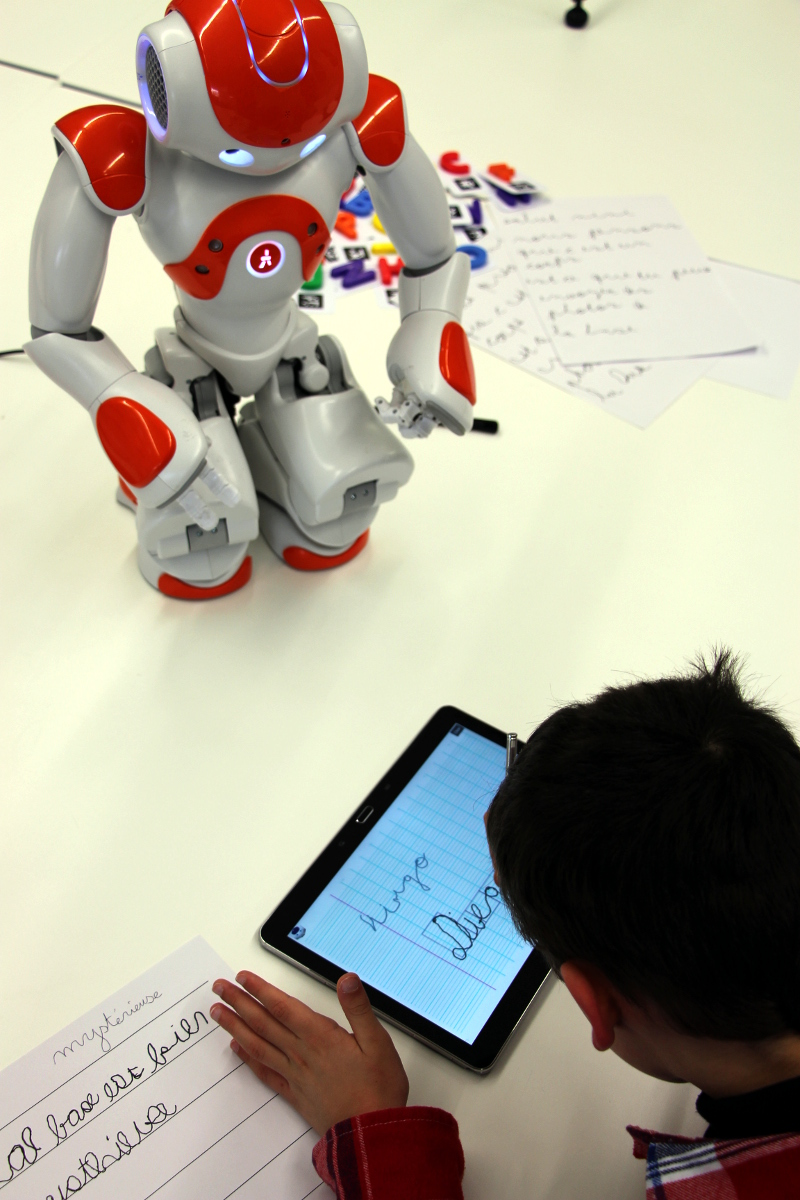
\includegraphics[width=0.7\linewidth]{cowriter}
    \end{center}

\end{multicols}
\end{frame}
\begin{frame}[plain]
    \begin{center}
        \Large
        \href{https://www.mentimeter.com/s/3ca728c0780550ff7296e7c31af2e317/b90ca40dfa36}{Go
        to www.menti.com and use the code 15 14 87}
    \end{center}
\end{frame}

\section[hacker\_space]{BRL's hacker\_space}

\imageframe[color=black]{hacker_space}


\begin{frame}{BRL's hacker\_space}

    \begin{itemize}
        \item \textbf{open 24/7 to students}
        \item lockers where to leave your projects
        \item dual-boot computers (with CAD software)
        \item soldering stations, scopes, basic tools
    \end{itemize}

    \begin{center}
        \Large
        \textbf{Make it your own!!}
    \end{center}

\end{frame}


\begin{frame}{During work hours...}
    \begin{itemize}
        \item Julian is around
        \item Access to the hacker\_space workshop (press drill, etc)
        \item Loads of kits are available (you need to sign them out): Arduinos,
            RaspberryPI, motors, servomotors, sensors (3D cameras, GPS, LIDARs... you name
            it!)
    \end{itemize}
\end{frame}

\imageframe[color=black]{hacker_space_workshop}

\section{A space for thinkering with crazy ideas}

\videoframe[0.56]{figs/projects/ROCO222-Robot-Arm-1st-demo-.3gpp.mp4}
\imageframe[color=black]{figs/projects/auto_maze}
\videoframe[0.56]{figs/projects/Gesture-controlled_Drone.3gpp.mp4}
\imageframe[color=black]{figs/projects/FinalMotor}
\imageframe[color=black]{figs/projects/3d_scanner}
\videoframe[0.56]{figs/projects/pothole_detection.webm}
\imageframe[color=black]{figs/projects/haptic_obstacle_detector}
\videoframe[0.56]{figs/projects/3D-printed-Robot-Arm-controlled-with-ROS.3gpp.mp4}
\videoframe[1.4]{figs/projects/IMU_RC_Car.mp4}
\videoframe[0.56]{figs/projects/gun_turret.mov}


\videoframe[0.56]{figs/NISSAN-ProPILOT-chair.mp4}


\begin{frame}{Module aims}
    \begin{itemize}
        \item<+-> Develop an in-depth understanding of \textbf{what electrical motors are},
            \textbf{how they work} (hands-on!), how they are characterised
        \item<+-> Learn how to \textbf{control them}, and \textbf{program an embedded controller}
            for your own motor
        \item<+-> Get a first \textbf{hand-on experience with a complete robotic system}:
            from the hardware, to the low-level closed-loop control, to
            system-level programming and visualisation
        \item<+-> \textbf{We have a bit of room to touch additional topics}
    \end{itemize}
\end{frame}

\begin{frame}{Learning outcomes}
    \begin{enumerate}
        \item<+-> Demonstrate knowledge and critical understanding of the operating
            \textbf{characteristics of electrical motors} (brushed, brushless,
            servo, stepper motors...)
        \item<+-> Explore (some) \textbf{robot sensors}, integrate them into software
        \item<+-> Comprehend and characterise the effects of \textbf{closing the speed and current
            loops} in drive systems; demonstrate it practically by \textbf{creating a
            closed loop motor system}
        \item<+-> Understand the fundamentals of the \textbf{ROS middleware},
            and use it to control motors and run simple robot visualisations
        \item<+-> Acquire the \textbf{basics of software engineering}; feel
            confident when using the \textbf{Linux command-line}; know how to
            use and reflect on \textbf{document/code versioning and sharing}
            (with git)

    \end{enumerate}
\end{frame}

\begin{frame}{In your curriculum}
    \begin{itemize}
        \item Last year: quite a lot of electronics, \textbf{ROCO103PP}?
        \item Next term: \textbf{ROCO224} (Martin Stoelen) -- kinematics, mechanical engineering,
            robot control
        \item Next year: \textbf{ROCO318} -- sensors, algorithms, AI (path
            planning, localisation)
    \end{itemize}
\end{frame}

\begin{frame}{This module: syllabus}

\begin{itemize}
    \item<+-> \textbf{Week 1} -- Arduino + Encoders
    \item<+-> \textbf{Week 2} -- The physics behind motors: electromagnetism, induction, magnetic
        force
    \item<+-> \textbf{Week 4} -- DC motors, brushed \& brushless
    \item<+-> \textbf{Week 5} -- Closed-loop motor control, PWM, PID, H-bridge
    \item<+-> \textbf{Week 6} -- Induction motors
    \item<+-> \textbf{Week 7} -- Servo-motors \& stepper motors
    \item<+-> \textbf{Week 9} -- Software engineering for robotics
    \item<+-> \textbf{Week 10} -- ROS middleware, joint state, kinematics 101, visualisation
    \item<+-> \textbf{Week 11} -- Sensors
\end{itemize}

\end{frame}



\end{document}
